\documentclass[12pt]{article}
\usepackage{../../ficha}

\begin{document}

\ficha{Funções Linear e Afim}[Referencial Cartesiano, Conceito de Função e Declive]

\instrucoes{Resolve os exercícios, apresentando os cálculos. Uma função afim tem expressão $f(x) = ax + b$, onde $a$ é o declive e $b$ a ordenada na origem; se $b = 0$, a função é linear.}

\secao{Referencial Cartesiano}{Observa o referencial e responde.}

\begin{center}
\begin{tikzpicture}[scale=0.55]
  \draw[very thin, gray!40] (-5,-4) grid (5,4);
  \draw[-{Latex}] (-5.3,0) -- (5.4,0) node[right] {$x$};
  \draw[-{Latex}] (0,-4.3) -- (0,4.4) node[above] {$y$};
  \foreach \i in {-4,-2,2,4} \node[below, font=\scriptsize] at (\i,0) {$\i$};
  \foreach \i in {-2,2} \node[left, font=\scriptsize] at (0,\i) {$\i$};
  \fill (3,2) circle (3pt) node[above right] {$A$};
  \fill (-2,3) circle (3pt) node[above left] {$B$};
  \fill (-4,-1) circle (3pt) node[below left] {$C$};
  \fill (1,-3) circle (3pt) node[below right] {$D$};
  \fill (0,-2) circle (3pt) node[left] {$E$};
  \fill (4,0) circle (3pt) node[above right] {$F$};
\end{tikzpicture}
\end{center}

\begin{exercicios}
  \item Indica as coordenadas dos pontos $A$, $B$, $C$, $D$, $E$ e $F$.
  \item Em que quadrante está cada um dos pontos $A$, $B$, $C$ e $D$?
  \item Quais dos pontos estão sobre os eixos coordenados?
  \item Indica as coordenadas do ponto simétrico de $A$ em relação ao eixo $Ox$.
  \item Indica as coordenadas do ponto simétrico de $B$ em relação à origem.
  \item Num referencial, marca os pontos $P(2,-3)$, $Q(-1,0)$ e $R(0,4)$.
\end{exercicios}

\secao{Conceito de Função}{Responde a cada questão.}
\begin{exercicios}
  \item A correspondência que a cada aluno associa a sua data de nascimento é uma função? E a que a cada data associa os alunos nascidos nesse dia?
  \item Considera $f : \{1, 2, 3, 4\} \to \R$ definida por $f(x) = 2x - 1$. Indica o domínio, o conjunto de chegada e o contradomínio.
  \item Para $f(x) = 3x + 2$, calcula $f(0)$, $f(2)$ e $f(-1)$.
  \item Para $g(x) = x^2 - 4$, calcula $g(3)$, $g(-3)$ e $g(0)$.
  \item Para $f(x) = 5x - 3$, determina $x$ de modo que $f(x) = 12$.
  \item Uma tabela tem os pares $(1, 3)$, $(2, 5)$, $(1, 4)$, $(3, 7)$. Representa uma função de $x$? Justifica.
  \item O preço de uma corrida de táxi é 3,25 euros mais 0,90 euros por km. Escreve a função $P(k)$ que dá o preço em função dos quilómetros $k$.
\end{exercicios}

\secao{Funções Lineares e Afins}{Para cada função, indica o declive e a ordenada na origem, e classifica-a como linear, afim ou constante.}
\begin{exercicios}
  \item $f(x) = 2x + 3$
  \item $g(x) = -x + 5$
  \item $h(x) = 4x$
  \item $i(x) = \dfrac{1}{2}x - 1$
  \item $j(x) = 7$
  \item $k(x) = -3x$
  \item $m(x) = 2(x - 1) + 5$
  \item Representa graficamente $f(x) = 2x + 1$ e $g(x) = -x + 4$ no mesmo referencial e indica o ponto de interseção.
\end{exercicios}

\secao{Declive e Equação da Reta}{Determina a expressão da função afim nas condições indicadas.}
\begin{exercicios}
  \item Declive 3 e ordenada na origem $-2$.
  \item Declive $-\dfrac{1}{2}$ e passa no ponto $(0, 4)$.
  \item Passa nos pontos $(0, 1)$ e $(2, 7)$.
  \item Passa nos pontos $(1, 5)$ e $(3, 9)$.
  \item Passa nos pontos $(-2, 6)$ e $(2, -2)$.
  \item É paralela a $y = 4x - 1$ e passa na origem.
  \item É paralela a $y = -2x + 3$ e passa no ponto $(1, 5)$.
  \item Calcula o declive da reta que passa por $A(-1, 3)$ e $B(4, -7)$.
\end{exercicios}

\secao{Interpretação de Gráficos}{Observa os gráficos das funções $f$ e $g$ e responde.}

\begin{center}
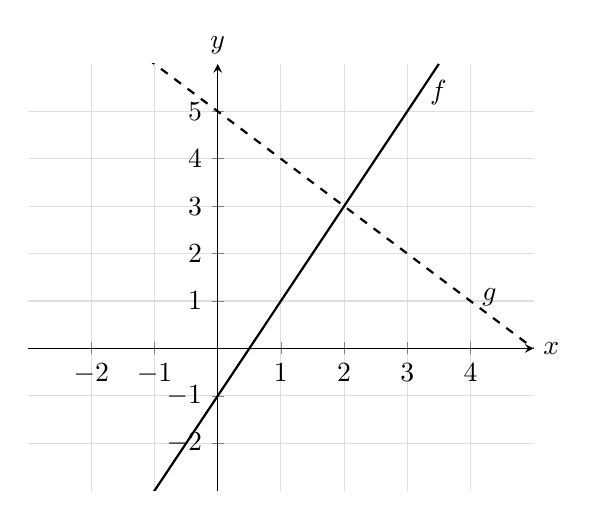
\begin{tikzpicture}
\begin{axis}[axis lines=middle, xmin=-3, xmax=5, ymin=-3, ymax=6, xtick={-2,...,4}, ytick={-2,...,5}, grid=both, grid style={gray!25}, width=8cm, height=7cm, xlabel=$x$, ylabel=$y$, every axis x label/.style={at={(ticklabel* cs:1)},anchor=west}, every axis y label/.style={at={(ticklabel* cs:1)},anchor=south}]
  \addplot[thick, domain=-2.5:3.5] {2*x - 1} node[pos=0.95, right] {$f$};
  \addplot[thick, dashed, domain=-3:5] {-x + 5};
  \node[above] at (axis cs:4.3,0.7) {$g$};
\end{axis}
\end{tikzpicture}
\end{center}

\begin{exercicios}
  \item Indica a ordenada na origem de $f$ e de $g$.
  \item Determina o declive de $f$ e o de $g$.
  \item Escreve a expressão algébrica de $f$ e de $g$.
  \item Determina as coordenadas do ponto de interseção dos dois gráficos.
  \item Para que valores de $x$ se tem $f(x) > g(x)$?
  \item Determina o zero de cada função.
\end{exercicios}

\secao{Desafios}{Resolve os problemas.}
\begin{exercicios}
  \item Um ginásio cobra 20 euros de inscrição e 25 euros por mês. Outro cobra 35 euros por mês sem inscrição. A partir de quantos meses é mais vantajoso o primeiro?
  \item Uma vela de 30\,cm arde 2\,cm por hora. Escreve a altura $h$ em função do tempo $t$. Ao fim de quanto tempo se apaga?
  \item Os pontos $(1, 2)$, $(3, 8)$ e $(5, k)$ estão na mesma reta. Determina $k$.
  \item Uma função afim verifica $f(2) = 5$ e $f(6) = 13$. Determina $f(10)$.
  \item Determina a área do triângulo formado pela reta $y = -2x + 6$ e pelos eixos coordenados.
\end{exercicios}

\end{document}
